\documentclass[11pt,letterpaper,english]{article}

\usepackage[margin=1.0in]{geometry}
\usepackage{helvetica}
\usepackage[table]{xcolor}
\usepackage{graphicx}

\title{Effects of Economic Relase Data on Market Health Indicators}
\author{Ian Clark}
\date{}

\begin{document}
\maketitle

\section{The ISM Manufacturing Index}
With a consensus range from 53.5 to 56.5 and a mean consensus of 55, the data for the ISM Manufacturing Index was released lower than predicted at 53.5. 

\subsection{Affects Upon the Market}
Affects upon the S\&P 500 were questionable at best, as the general economic climate was already slipping into turmoil because of news concerning the European Central Bank and decisions from Greece's new Finance Minister Yanis Varoufakis. Regardless, operating under the (naïve) assumption that a negative/positive change in the ISM Manufacturing Index would negatively/positively affect the S\&P 500, we can see correlation--$\Delta{ISM} = -1.6$ and $\Delta{S\&P} = -15.77$ or $\%\Delta{S\&P} = -0.79$. Admittedly, these numbers are opening and low amounts and the S\&P index ended the day on a net gain in value.

\section{The Employment Situation}
The employment situation data has all-around been fantastic, with consistently high revisions ranging from November's astounding revisions in Non-farm month-to-month Payroll to February's release data. Considering the trend (please see below data), further positive revisions seem both feasible and plausible.

\begin{center}
    \begin{tabular}{| c | c | c | c |}
    \hline
    Month       & Original (1000s) & Revised (1000s) & Difference (1000s) \\ \hline
    November    & 353 & 423 & \cellcolor{green}{+70} \\ \hline
    December    & 252 & 329 & \cellcolor{green}{+77} \\ \hline
    January     & 321 & 353 & \cellcolor{green}{+32} \\ \hline
    February    & 257 & \cellcolor{black}{} & \cellcolor{black}{} \\ \hline
    \end{tabular}
\end{center}

Moreover, the Unemployment Level (the u3) has risen (employment has increased) from 5.6\% to 5.7\%, albeit this seems to indicate the economy is in such a promising position that many previously discouraged workers have opted to return to the job search, thus creating a slight convergence between the u3 and u6 employment rates. 
Contributing to this, we saw a rise from 62.7\% labor force participation to 62.9\%. This statistic, however, is not as impressive, as the trend has been for labor force participation to remain near 62.9\%, as seen below:

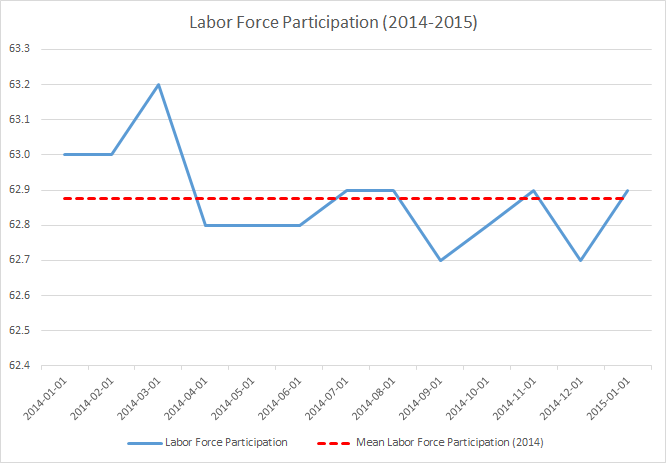
\includegraphics[scale=0.85]{LaborForceParticipation.png}
\vspace{5mm}

As well, the other promising statistic within the data is the month-to-month Average Hourly Earnings, which rose a total of .5\%--exceeding the consensus range (.1\% to .5\%) by an entire 20\%. From September to December of 2014, the United States experienced positive net gains across all workers\footnote[1]{ The Employment Cost Index, http://www.bls.gov/web/eci/ecconstnaics.txt}, so for the foreseeable future, this trend may well continue.

\subsection{Effects Upon the Market}
Given the positive nature of the Employment Situation data, one could reasonably assume positive gains within the S\&P 500, as these numbers can sensibly predict growth within the economy. As such, one could operate under the (naïve) assumption that when the news is positive, so is the reaction upon the market. The high of February 6\textsuperscript{th} for the S\&P 500 was 2072.4, yet the market opened at 2062.28. While the employment numbers may have had a positive effect on the S\&P 500 for a duration, the duration was not long-lasting as the S\&P 500 closed at 2055.47--a loss for the day of 0.33\%.


\end{document}